\documentclass[14pt]{scrartcl}
\usepackage{amsmath}
\usepackage{graphicx}
\usepackage{geometry}
\usepackage{fancyhdr}
\usepackage{caption}
\usepackage{subcaption}
\usepackage{hyperref}
\usepackage[nottoc,notlof,notlot]{tocbibind} 
\usepackage{comment}
\graphicspath{ {./pictures/} }
\linespread{1.6}
\geometry{
		left=3cm,
		right=1cm,
		top=2cm,
		bottom=2.5cm
}
\begin{document}
	\begin{titlepage}
		\pagestyle{fancy}
		\begin{center}
			O`ZBEKISTON RESPUBLIKASI\\ OLIY VA O`RTA-MAXSUS TA'LIM VAZIRLIGI\\
			MIRZO ULUG`BEK NOMIDAGI\\ O`ZBEKISTON MILLIY UNIVERSITETI\\
			FIZIKA FAKULTETI
		\end{center}
	\vfill
	\begin{center}
		\textsc{\Huge{KURS ISHI}}
	\end{center}

\begin{center}
	\textrm{\Large {Koinotning birinchi daqiqalari. Barion asimmetriyasi}}
\end{center}
\vfill
\begin{flushleft}
	\textbf{Bajardi}: F/18-06 guruh talabasi Urakbayeva O`.
	
	\textbf{Qabul qildi}: f.-m.f.d., prof. Polvonov S.R.
\end{flushleft}

\vfill
\vfill
\begin{center}
	\texttt{Toshkent, 2021}
\end{center}
	\end{titlepage}
\renewcommand{\abstractname}{Kirish}
\renewcommand{\contentsname}{Mundarija}
\tableofcontents
\addcontentsline{toc}{section}{Kirish}
\newpage
\section*{Kirish}
\hspace{0.6cm}Katta portlash (inglizcha: Big Bang) nazariyasi amaldagi kosmologik model bo`lib, olam rivojlanishining erta bosqichlarini tasvirlaydi. Bu nazariyaga binoan Katta portlash taxminan 13,798 $\pm$ 0.037 milliard yil oldin sodir bo`lgan; bu ko`rsatkich olam yoshi deb hisoblanadi. Bundan keyin olam o`ta issiq va zich holatda bo`lib, keskin kengayishni boshlagan. Boshlang`ich kengayishdan so`ng olam energiyaning turli subatom zarrachalar, jumladan proton, neytron va elektronlarga aylanishi uchun yetarli darajada sovugan. Sodda atom yadrolari tezda shakllangan bo`lishi mumkin, biroq birinchi elektrik neytral atomlar yuzaga kelishi uchun minglab yillar kerak bo`lgan. Kimyoviy unsurlardan birinchi bo?lib vodorod, keyin geliy va litiy hosil bo`lgan. Ushbu ibtidoiy unsurlarning ulkan bulutlari keyinchalik gravitatsiya orqali yulduz va galaktikalarni shakllantirish uchun yig`ilgan; og`irroq unsurlar esa yulduzlarda yoki o`ta yangi yulduzlar portlashlarida sintezlangan.

Katta portlash sinchiklab tekshirilgan ilmiy nazariya hisoblanadi va u ilmiy hamjamiyat tomonidan keng qabul qilingan. U yengil unsurlar ko`pligi, qoldiq nurlanish, koinot tuzilishi va Ia tipli o`ta yangi yulduzlarning Hubble diagrammasi kabi kuzatiladigan turli fenomenlarni batafsil izohlaydi. Katta portlash-ning negiz g`oyalari - kengayish, erta issiq holat, geliy va galaktikalar shakllanishi - bu va boshqa kuzatishlardan kelib chiqib, har qanday kosmologik modeldan mustaqildir. Galaktika to`plamlari orasidagi masofalar hozirda kattalashib bori-shidan o`tmishda hamma narsa bir-biriga yaqinroq bo`lgani haqidagi xulosaga olib kelgan. Bu g`oya ekstremal zichlik va haroratlargacha olib borilib, bunday holatlarda tajribalar olib borish uchun katta zarracha tezlatgichlari qurilgan, natijada bu ilmiy model to`liqroq ishlab chiqilgan. Boshqa tomondan, bu tezlatgichlarning o`ta yuqori energiyalar fizikasini tadqiq qilish uchun qobiliyatlari cheklangan. Kengayishning mutlaq ilk lahzasiga oid dalillar juda kam. Shunday qilib, Katta portlash nazariyasi bu ilk holatni izohlay olmaydi; biroq u olamning shu lahzadan keyingi umumiy evolutsiyasini tasvirlaydi va tushuntiradi.

Katta portlash nazariyasi ildizlari Georges Lema\^{i}tre tomonidan o`rtaga tashlangan "ibtidoiy atom gipotezasiga" borib taqaladi. Vaqt o`tishi bilan olimlar uning g`oyalari asosida zamonaviy sintez nazariyasini qurishdi. Katta portlash modeli Albert Einstein'ning umumiy nisbiylik nazariyasi va fazoning bir xilligi va izotropiyasi kabi tushunchalarga tayanadi. Asosiy tenglamalar Aleksandr Fridman tomonidan ta'riflangan. 1929-yili Edwin Hubble uzoq galaktikalargacha masofalar ularning qizil siljishiga mutanosib ekanini aniqladi - bu g`oya Lema\^{i}tre tomonidan 1927-yili olg`a surilgan edi. Hubblening kuzatuvi barcha uzoq galaktika va klasterlar kuzatuv nuqtamizdan qochayotgan ko`rinma tezlikka ega ekanini ko`rsatdi: galaktika qancha uzoq bo`lsa, ko`rinma tezligi shunchalik yuqori.

Ilmiy hamjamiyat bir vaqtlar Katta portlash va Sobit olam nazariyalari tarafdorlariga ajralgan bo`lsa, 1964-yil qoldiq nurlanish kashfiyoti va ayniqsa u-ning spektri (ya'ni, har to`lqin uzunligida o`lchangan nurlanish miqdori) mutlaq qora jism issiqlik nurlanishiga mos kelishi aniqlanganidan keyin ko`pchilik olimlar kuzatuvlarga Katta portlash ssenariylaridan biri eng mos kelishiga iqror bo`lishdi. Shundan buyon Lambda-CDM modeli zamonaviy nazariy kosmologiya tadqiqotlari tuzilmasi bo`lib xizmat qilgani uchun astrofiziklar Katta portlash modeli va uning parametrizatsiyasiga keng ko`lamli kuzatuv va nazariy qo`shim-chalar qilishdi. 
\newpage
\section{Asosiy qism}
\subsection{Katta portlash nazariyasining paydo bo`lishi}
\hspace{0.6cm}
Katta portlash nazariyasi olam tuzilishini kuzatish va nazariy muhokamalardan kelib chiqqan. 1912-yilda Vesto Slipher birinchi bo`lib spiral galaktika (u paytda "spiral tumanlik" deyilar edi) Doppler siljishini o`lchadi va deyarli barcha shunday tumanliklarning Yerdan chekinayotganini aniqladi. U bu faktning kosmologik ahamiyatini payqamadi, zero XX asr boshida bu tumanliklar Somon yo`li ichida yoki tashqarisida ekanligi bahsli savol edi.  O?n yil o`tib, rossiyalik kosmolog va matematik Aleksandr Fridmann Einstein tenglamalaridan yangi, Einstein yoqlab chiqqan sobit olam modelidan farq qilib, olamning kengayayotgan bo`lishi mumkinligini ko`rsatuvchi Fridmann tenglamalarini keltirib chiqardi.  1924-yilda Edwin Hubble spiral tumanliklargacha masofani o`lchab, bu tizimlarning aslida mustaqil galaktikalar ekanligini ko`rsatdi. 1927-yili Fridmanndan mustaqil ravishda belgiyalik fizik va katolik ruhoniy Georges Lema\^{i}tre tumanliklarning chekinishi olam kengayishi tufayli sodir bo`layotgani haqidagi farazni taklif qildi. 

1931-yilda Lema\^{i}tre fikrini yana rivojlantirib, olamning ayon kengayishi vaqt bo`ylab teskari proyeksiyalansa, ya'ni qancha ortga qaytilsa, olam shunchalik kichik bo`lishidan kelib chiqib chekli o`tmishda olam massasining bari "ibtidoiy atom" degan bir nuqtada jamlanib, u yerda vaqt va fazo yuzaga kelganini aytish mumkin, degan farazni taklif qildi. 

1924-yildan Hubble Mount Wilson observatoriyasidagi 2 500 mm Hooker teleskopi yordamida astronomik masofalar shkalasini boshlab bergan masofa ko`rsatkichlarini puxtalik bilan ishlab chiqa boshladi. Bu unga qizil surilishlari o`lchab bo`lingan galaktikalargacha masofalarni chamalashga imkon berdi. 1929-yilda Hubble masofa va chekinish tezligi orasida mutanosiblik topdi, hozirda bu mutanosiblik Hubble qonuni deb nomlanadi.  Lema\^{i}tre kosmologik prinsipdan kelib chiqib, bu mutanosiblikni oldindan bashorat qilgan edi. 

1920-1930-yillarda deyarli barcha yirik kosmologlar Sobit olam nazariyasiga yon bosib, ayrimlar Katta portlash nazariyasidan kelib chiqadigan vaqt ibtidosi diniy qarashlarni fizikaga ko`chirishdir, deb norozilik bildirgan; bu e'tiroz keyinchalik Sobit olam nazariyasi tarafdorlari tomonidan takrorlangan edi.  Bu norozilik Katta portlash nazariyasi mualliflaridan biri Georges Lema\^{i}tre katolik ruhoniy bo`lgani uchun yanada kuchaygan edi.  Arthur Eddington Arastuning olamning vaqtdagi boshlanishi yo`q, ya'ni materiya abadiydir, degan fikriga qo`shilgan. Vaqt ibtidosi haqidagi g`oya unga zid kelgan.  Biroq Lema\^{i}tre shunday fikr bildirgan:

\begin{quote}\texttt{Agar olam yagona kvant bilan boshlangan bo`lsa, fazo va vaqt tushunchalari ibtidoda ma'nosiz bo`lar edi; ular boshlang`ich kvant yetarli miqdordagi kvantlarga bo`linganidagina ma'noga ega bo`lishi mumkin. Agarda bu iddao to`g`ri bo`lsa, olam boshlanishi fazo va vaqt boshlanishidan biroz avval sodir bo`lgan.} 
\end{quote}
1930-yillarda Hubble kuzatuvlarini izohlash uchun nostandart kosmologiyalar sifatida boshqa g`oyalar, jumladan, Milne modeli, siklik olam (Fridman tomonidan ilgari surilgan, keyinchalik Albert Einstein va Richard Tolman e'tiborini qozongan) va Fritz Zwicky'ning charchagan yorug`lik gipotezalari paydo bo`ldi.

\subsection{Koinotning kengayishi}
\hspace{0.6cm}
\subsection{Birlamchi nukleosintez}
\hspace{0.6cm}
	\renewcommand{\arraystretch}{1.8}
\begin{center}
	\begin{tabular}{c c c}
		$n^{0}\rightarrow p^{+} + e^{-} + \overline{\nu}_{e}$&\ \ &$p^{+}+n^{0}\rightarrow^{2}_{1}\textrm{D} +\gamma$\\
		$^{2}_{1}\textrm{D}+p^{+}\rightarrow ^{3}_{2}\textrm{He}+\gamma$&\ \ &$^{2}_{1}\textrm{D}+^{2}_{1}\textrm{D}\rightarrow ^{3}_{2}\textrm{He}+n^{0}$\\
		$^{2}_{1}\textrm{D}+^{2}_{1}\textrm{D}\rightarrow ^{3}_{1}\textrm{T}+p^{+}$&\ \ &$^{3}_{1}\textrm{T}+^{2}_{1}\textrm{D}\rightarrow ^{4}_{2}\textrm{He}+n^{0}$\\
		$^{3}_{2}\textrm{He}+^{4}_{2}\textrm{He}\rightarrow ^{7}_{3}\textrm{Li}+\gamma$&\ \ &$^{3}_{2}\textrm{He}+n^{0}\rightarrow ^{3}_{1}\textrm{T}+p^{+}$\\
		$^{3}_{2}\textrm{He}+^{2}_{1}\textrm{D}\rightarrow ^{4}_{2}\textrm{He}+p^{+}$&\ \ &$^{3}_{2}\textrm{He}+^{4}_{2}\textrm{He}\rightarrow ^{7}_{4}\textrm{Be}+\gamma$\\
		$^{7}_{3}\textrm{Li}+p^{+}\rightarrow ^{4}_{2}\textrm{He}+^{4}_{2}\textrm{He}$&\ \ &$^{7}_{4}\textrm{Be}+n^{0}\rightarrow ^{7}_{3}\textrm{Li}+p^{+}$\\
	\end{tabular}
\end{center}
\subsection{Plank davri}
\hspace{0.6cm}
Plank davri -- kosmologik nazariyaga binoan, olam evolyutsiyasining portlashdan keyingi eng birinchi davri hisoblanadi. Ushbu davr noldan (ya'ni portlash ro`y bergan vaqtdan) $10^{-43}$ s gacha bo`lgan vaqtni o`z ichiga oladi. Ushbu davrda, taxminan 13,8 mlrd yil oldin materiya Plank energiyasi ( $10^{19}$ GeV), Plank radiusi ($10^{-35}$m) , Plank temperaturasi (10$^{32}$ K ) hamda Plank zichligi ($\sim10^{97}$g/sm$^{3}$) ga ega bo`lgan.

Olamning o`lchami juda kichik bo`lganligi tufayli, gravitatsiya kuchlari qolgan fundamental ta'sir kuchlari bilan birlasha olgan. Natijada gravitatsiyaning kvant effektlari qolgan fizik ta'sirlashuv kuchlaridan ustunlik qilgan. Biroq temperatura va zichlikning haddan tashqari katta qiymatga ega ekanligi tufayli, simmetriya buzilgan, natijada gravitatsion ta'sir qolgan fundamental ta'sir kuchlaridan ajralib qolgan. 

Zamonaviy kosmologiya nazariyasi bo`yicha Plank davridan so`ng, olam rivojlanishining ikkinchi fazasi -- Buyuk Birlashish Davri boshlangan. Undan so`ng esa Kosmik inflatsiya davri boshlangan. Ushbu davrda qisqa vaqt ichida olamning o`lchamlari juda tez o`zgargan, ya'ni kengaygan.


\subsection{Buyuk birlashish yoki supersimmetriya davri}
\hspace{0.6cm}
Buyuk Birlashish Davri - olam rivojlanishining ikkinchi fazasini tavsiflash uchun kiritilgan tushuncha. Olam kosmologik modeliga binoan, buyuk birlashish davri portlashdan $\sim 10^{-43}$ s o`tib boshlangan, bu vaqtda modda zichligi $10^{92}$ g/sm$^{3}$ ni tashkil etgan. Temperatura esa $10^{32}$ K ga teng bo`lgan. 


\subsection{Barion asimmetriyasi}
\hspace{0.6cm}
Barion asimmetriyasi -- olamning ko`zga ko`rinadigan qismida materiyaning antimateriyadan ustunlik qilishi. Ushbu faktni standart model bilan ham, umumiy nisbiylik nazariyasi bilan ham tushuntirishning imkoni yo`q. Shu sababli ushbu hodisa kosmologiyadagi hal qilinmagan muammolardan biri hisoblanadi.

1967-yili A.D.Saxarov chop etgan maqolada barion asimmetriyasi mavjud bo`lishi uchun zarur bo`lgan bir qancha shartlar keltirilgan:
\begin{itemize}
	\item olam va antiolam o`rtasidagi asimmetriya, buni ilmiy tilda C- va CP-simmetriyaning buzilishi deb ataladi;
	\item barion zaryadi saqlanish qonunining buzilishi;
	\item olam shakllanishining dastlabki bosqichlarida termodinamik muvozanatning buzilishi
\end{itemize}

Olam asimmetriyasining o`lchovi sifatida quyidagi kattalik ishlatiladi:
\begin{equation}
\delta=\frac{n-\tilde{n}}{n_{\gamma}}
\label{1}
\end{equation}
bu yerda $n$, $\tilde{n}$ va $n_{\gamma}$ - barionlar, antibarionlar va reliksion fotonlarning konsentratsiyalari. Ushbu fotonlarning konsentratsiyasi bizga ma'lum, ya'ni $T\approx3K$ haroratga mos kelgan konsentratsiyasi $n_{
\gamma} = 500 sm^{-3}$. Barion zaryadi konsentratsiyasi galaktikadagi ko`rinadigan materiya massasi tufayli chegaralangan: $n>3\cdot10^{-8}sm^{-3}$. U holda, $\delta = 10^{-8} - 10^{-10}$ tartibida bo`ladi. Olamning adiabatik kengayishida $\delta$ kattalik vaqtga kuchsiz bog`liq[10]. 


Barion asimmetriyasining vujudga kelishi mexanizmini quyidagicha tushuntirish mumkin. Buyuk birlashish nazariyasiga binoan, tabiatda leptokvarklar (X) - barion zaryadi saqlanmagan holda ro`y beradigan o`zaro ta'sirda qatnashadigan zarralar mavjud. Vektor leptokvarklarning massasi $M_{X}\approx10^{14} - 10^{18}GeV$, skalyar leptokvarklarning massalari esa $\approx10^{10}-10^{15}GeV$ tartibida bo`ladi. C- va CP- invariantlikning buzilishi, shuningdek, leptokvarklarning parchalanishida barion zaryadining saqlanmasligi tufayli kvarklar (q) va leptonlar (l), antikvark ($\tilde{q}$) hamda antileptonlar ($\tilde{l}$) ga nisbatan ko`proq hosil bo`ladi. Materiyaning zaryad simmetriyasiga ega qismi, koinot rivojlanishining keyingi bosqichlarida foton, neytrino va antineytrinoga parchalanib ketadi. Natijada faqatgina asimmetrik qism qoladi. 
\renewcommand{\figurename}{-rasm.}
\begin{figure}
	\centering
	\begin{subfigure}{.5\textwidth}
		\centering
		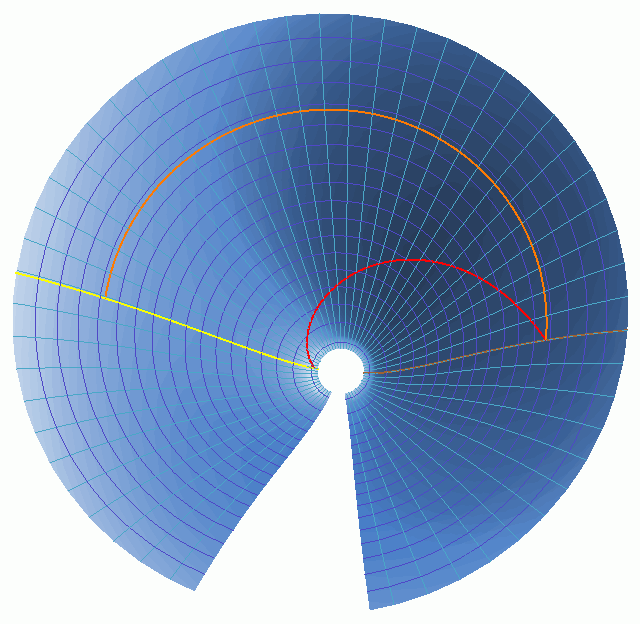
\includegraphics[width=0.7\linewidth]{pictures/Embedded_LambdaCDM_geometry_(alt_view)}
		\caption{Vertikal proyeksiya}
	\label{fig:embeddedlambdacdmgeometryaltview}
	\end{subfigure}%
	\begin{subfigure}{.5\textwidth}
		\centering
		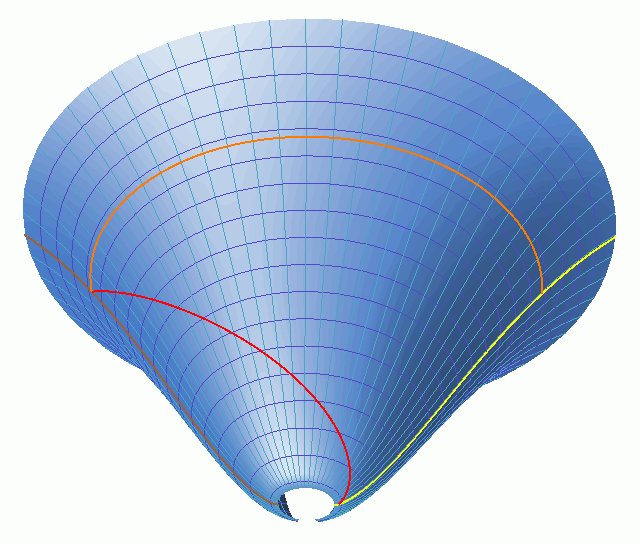
\includegraphics[width=0.7\linewidth]{pictures/Embedded_LambdaCDM_geometry}
		\caption{Gorizontal proyeksiya}
		\label{fig:embeddedlambdacdmgeometry}
	\end{subfigure}
	1-rasm.
	\textit{Olam ko`zga ko`rinadigan qismining izometrik tasviri. Ushbu tasvir orqali yorug`lik nuri (qizil chiziq), qanday qilib 13 milliard yil ichida 28 milliard yorug`lik yiliga teng bo`lgan masofani (zarg`aldoq chiziq) bosib o`tishi mumkinligini ko`rish mumkin.}
	\label{fig:test}
\end{figure}




Tasavvur qilaylik, bitta leptokvark (X) bor bo`lsin. Ushbu leptokvark ikkita antikvarkka yoki kvark va leptonga parchalanishi mumkin. Ushbu zarralarning parsial kengliklari mos holda $\Gamma_{1}$ va $\Gamma_{2}$ bo`lsin. U holda X zarraning parchala-nishida hosil bo`ladigan barion zaryad quyidagiga teng bo`ladi:
\begin{equation}
B_{X} = \frac{1}{\Gamma_{um}}\left(\frac{1}{3}\Gamma_{2} -\frac{2}{3}\Gamma_{1}\right)
\label{2}
\end{equation}

bu yerda $\Gamma_{um}$ - parchalanishning umumiy kengligi.

$\tilde{X}\rightarrow qq$ yoki $X\rightarrow\tilde{q}l$ sxema bo`yicha parchalanadigan antileptokvark uchun esa:
\begin{equation}
B_{\tilde {X}} = \frac{1}{\Gamma_{um}}\left(-\frac{1}{3}\tilde{\Gamma}_{2} +\frac{2}{3}\tilde{\Gamma}_{1}\right)
\label{3}
\end{equation}

CPT - invariantlikka binoan, $\Gamma_{um} \equiv \Gamma_{1} +\Gamma_{2}=\tilde{\Gamma}_{1}+\tilde{\Gamma}_{2}$.

Biroq, C- va CP-invariantlikning saqlanmasligi tufayli, $\Gamma_{1}\neq \tilde{\Gamma}_{1}$. Shu sababli, mikroskopik asimmetriya:
\begin{equation}
\delta_{micro}\equiv\frac{1}{2}\left(B_{X}+B_{\tilde{X}}\right) = 
\frac{\Gamma_{1}-\tilde{\Gamma}_{1}}{\Gamma_{um}}\neq 0
\label{4}
\end{equation}

Makroskopik asimmetriya esa $\delta\approx\frac{0,1}{N}\delta_{micro}\cdot S$ tartibida bo`ladi.

bu yerda $N$ - barcha zarralarning erkinlik darajalari, $S$ - makroskopik faktor bo`lib, ushbu faktor leptokvarklarning parchalanishiga simmetrik plazmaning ta'sirini hisobga oladi.

Biz ko`rib chiqayotgan hol uchun:


\begin{equation}
	S \approx  \begin{cases} 1, & \mbox{agar } \xi \le 1\\ \frac{0,2}{\xi \ln{\xi}}, & \mbox{agar } \xi > 1 \end{cases}
	\end{equation}
	
	bu yerda $\xi=\Gamma_{um}\cdot\frac{M_{0}}{M^{2}_{X}}$, $M_{0}=\frac{M_{Pl}}{1,66\cdot N^{1/2}}$ ($M_{Pl}=1,2\cdot 10^{19}$GeV - Plank massasi). $\xi \le 1$ da leptokvarklarning parchalanishi nosimmetrik bo`ladi va shu sababli ortiqcha barion zaryadi keyingi davrgacha saqlanib qoladi. $\xi \ge 1$ bo`lganda esa, parchalanish jarayonidagi termodinamik muvozanatning saqlanishi barion zaryadining kamayishiga olib keladi. 
\renewcommand{\refname}{Foydalanilgan adabiyotlar}
\newpage
\addcontentsline{toc}{section}{Xulosa}
\section*{Xulosa}
\newpage
\begin{thebibliography}{10}
	\bibitem[1]{1}{\textit{Asad, Muhammad}. The Message of the Qur'an. - Gibraltar, British Overseas Territory: Dar al-Andalus Limited, 1980.}
	\bibitem[2]{2}{\textit{Belu\^{s}evi\'{c}, Radoje.} Relativity, Astrophysics and Cosmology. - Weinheim: Wiley-VCH, 2008.}
	\bibitem[3]{3}{ \textit{Gibson, C.H.} (2001). "Turbulence And Mixing In The Early Universe".}
	\bibitem[4]{4}{\textit{Peter Goldreich}, Yoram Lithwick, Re'em Sari. Final Stages of Planet Formation // The Astrophysical Journal : journal. - IOP Publishing, 2004. }
	\bibitem[5]{5}{\textit{William F. Bottke, Daniel D. Durda, David Nesvorny et al.} Linking the collisional history of the main asteroid belt to its dynamical excitation and depletion // Icarus : journal. - Elsevier, 2005.}
	\bibitem[6]{6}{\textit{Woolfson, Michael}. Time, Space, Stars \& Man: The Story of Big Bang - London: Imperial College Press, 2013}
	\bibitem[7]{7}{\textit{Yao, W.M}. Review of Particle Physics// Journal of Physics G: Nuclear and Particle Physics : journal. - Bristol: IOP Publishing, 2006. - Vol. 33, }
	\bibitem[8]{8}{\textit{Allday, Jonathan.} Quarks, Leptons and the Big Bang. - Institute of Physics Publishing, 2001.}
	\bibitem[9]{9}{\textit{Lyth, David H.; Riotto, Antonio} (1999). ?Particle physics models of inflation and the cosmological density perturbation?. Physics Reports. }

\end{thebibliography}
\end{document}
